\section{Reanalysis of bow shock sources from Kobulnicky et al. (2016,
  2017, 2018)}
\label{app:bow-shock-data}

In a series of papers \citeauthor{Kobulnicky:2018a} provide an
extensive mid-infrared-selected sample of over 700 candidate stellar
bow shock nebulae (\citealp{Kobulnicky:2016a, Kobulnicky:2017a,
  Kobulnicky:2018a}, hereafter K16, K17, and K18).  For 20 of these
sources, reliable distances and spectral classifications are provided
(Table~5 of K17 and Tables~1 and~2 of K18), and these are used in
\S~\ref{sec:summary-discussion}, where we discuss the
\(\tau\)--\(\eta\) diagnostic diagram.  In this appendix, we outline our
treatment and analysis of the data in these catalogs, which differs in
some important respects from that of the original authors.

The UV optical depth of the bow shell is obtained
(eq.~[\ref{eq:tau-empirical}]) from the ratio of infrared shell
luminosity to stellar luminosity.  The inverse of this ratio is given
in Table~5 of K17, but we choose to re-derive the values since the
spectral classification of some of the sources was revised between K17
and K18.  Although K17 found the total shell fluxes from fitting dust
emission models to the observed SEDs, we adopt the simpler approach of
taking a weighted sum of the flux densities \(F_\nu\) (in \si{Jy}) in
three mid-infrared bands:
\begin{multline}
  \label{eq:total-ir-flux}
  F_{\text{IR}}  \approx \bigl[  2.4\,(F_8 \text{ or } F_{12})
    + 1.6\,(F_{22} \text{ or } F_{24})  \\
  + 0.51\,F_{70}\bigr]
  \,\times \SI{e-10}{erg.s^{-1}.cm^{-2}} \ ,
\end{multline}
where \(F_8\) is Spitzer IRAC \SI{8.0}{\um}, \(F_{24}\) is Spitzer
MIPS \SI{23.7}{\um}, \(F_{12}\) and \(F_{22}\) are WISE bands 3 and 4,
and \(F_{70}\) is Herschel PACS \SI{70}{\um}.  The weights are chosen
so that the integral \(\int_0^\infty F_\nu \,d\nu\) is approximated by the sum
\(\Sigma_k F_k\, \Delta\nu_k\), under the assumption that fluxes in shorter (e.g.,
IRAC \SI{5.8}{\um}) and longer (e.g., PACS \SI{150}{\um}) wavebands
are negligible.  Shell fluxes are converted to luminosities using the
assumed distance to each source, and stellar luminosities are taken
directly from K18 Table~2, based on spectroscopic classification and
the calibrations of gravity and effective temperature from
\citet{Martins:2005a}.  

\begin{figure}
  \centering
  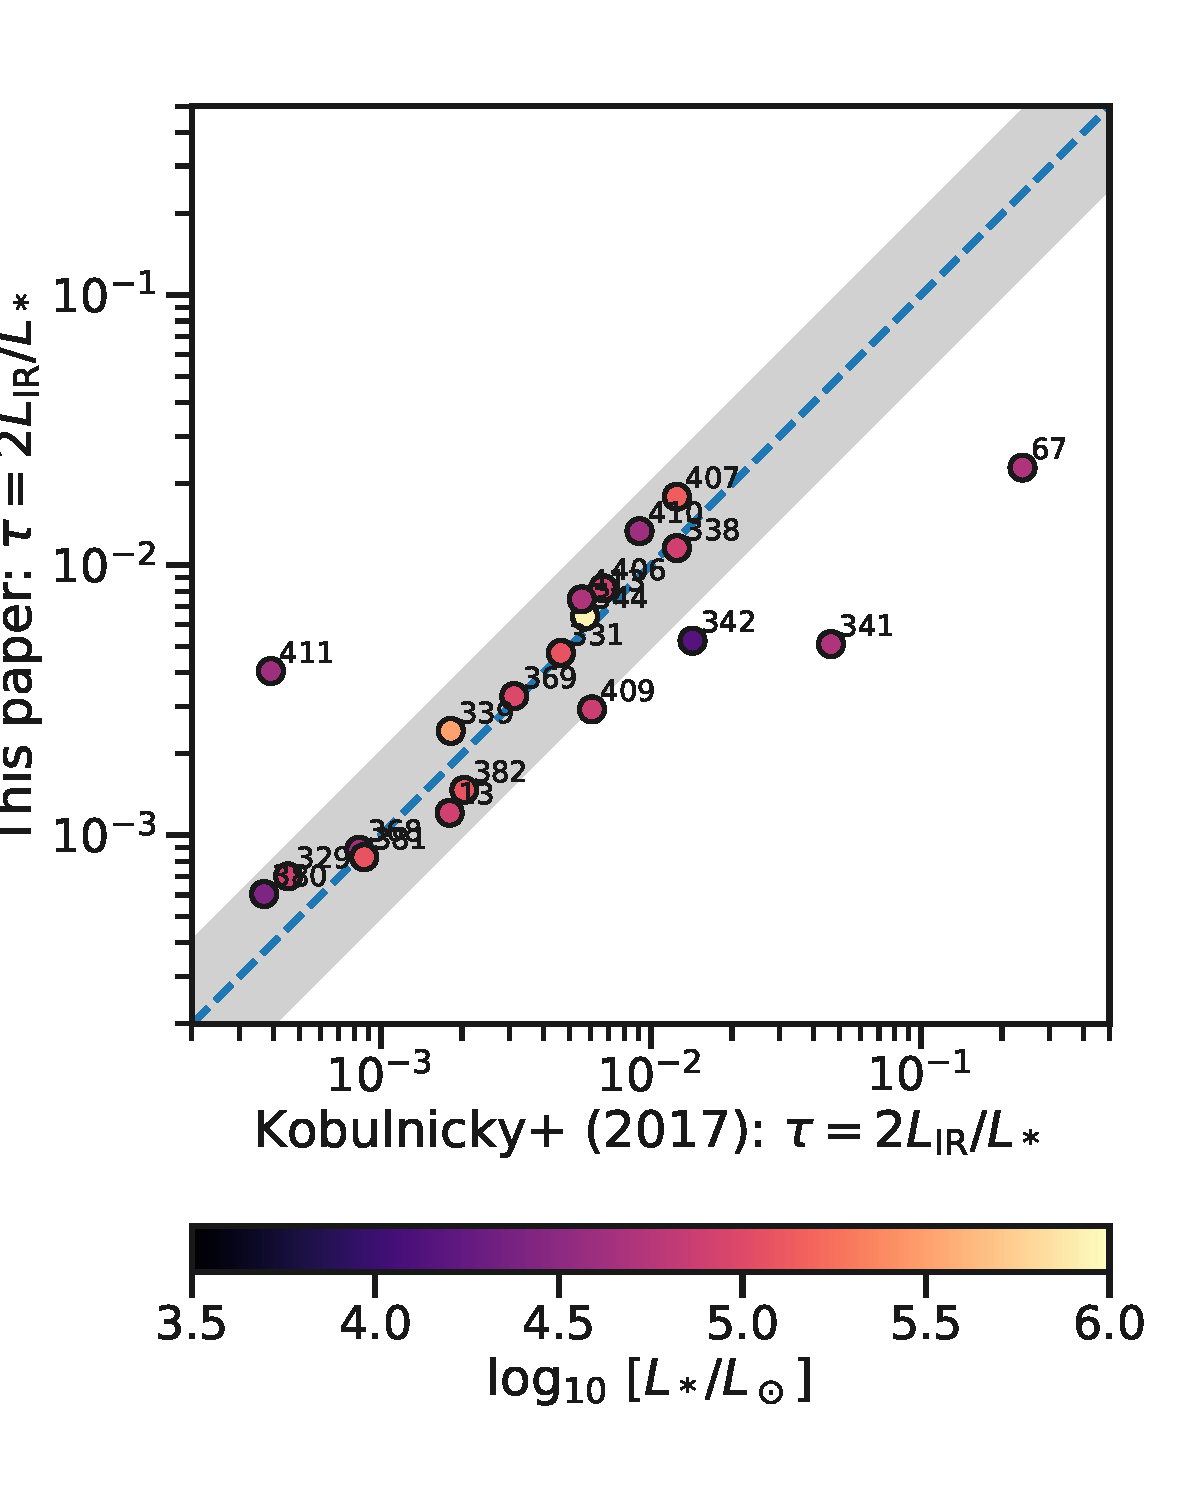
\includegraphics[width=\linewidth]{figs/K17-tau-comparison}
  \caption{Comparison between shell-to-star luminosity ratios
    calculated as described in the text (\(y\) axis) with those given
    in K17 (\(x\) axis).  The blue dashed line signifies equality and
    the gray band shows ratios between 1/2 and 2.}
  \label{fig:k17-k18-comparison}
\end{figure}

In Figure~\ref{fig:k17-k18-comparison} we compare the \(\tau\) obtained
using the shell luminosity as described above with that obtained using
the luminosity ratios directly from K17 Table~5.  It can be seen that
for the majority of sources the two measurements are consistent within
a factor of two (gray band).  The four furthest-flung outliers can be
understood as follows:
\begin{description}
\item[\textit{Source 67}] This has a very poor-quality spectral fit in
  K17 (see lower left panel of their Fig.~12) and so 
  \(F_{\text{IR}}\) is overestimated by them by a factor of 10.
\item[\textit{Sources 341 and 342}] The spectral classes changed from
  B2V in K17 to O9V and B1V, respectively, in K18, increasing the
  derived \(L_*\), which lowers \(\tau\).
\item[\textit{Source 411}] The luminosity class changed from Ib (K17)
  to V (K18), so \(L_*\) has been greatly reduced, which increases
  \(\tau\).
\end{description}

% \begin{figure*}
%   \centering
%   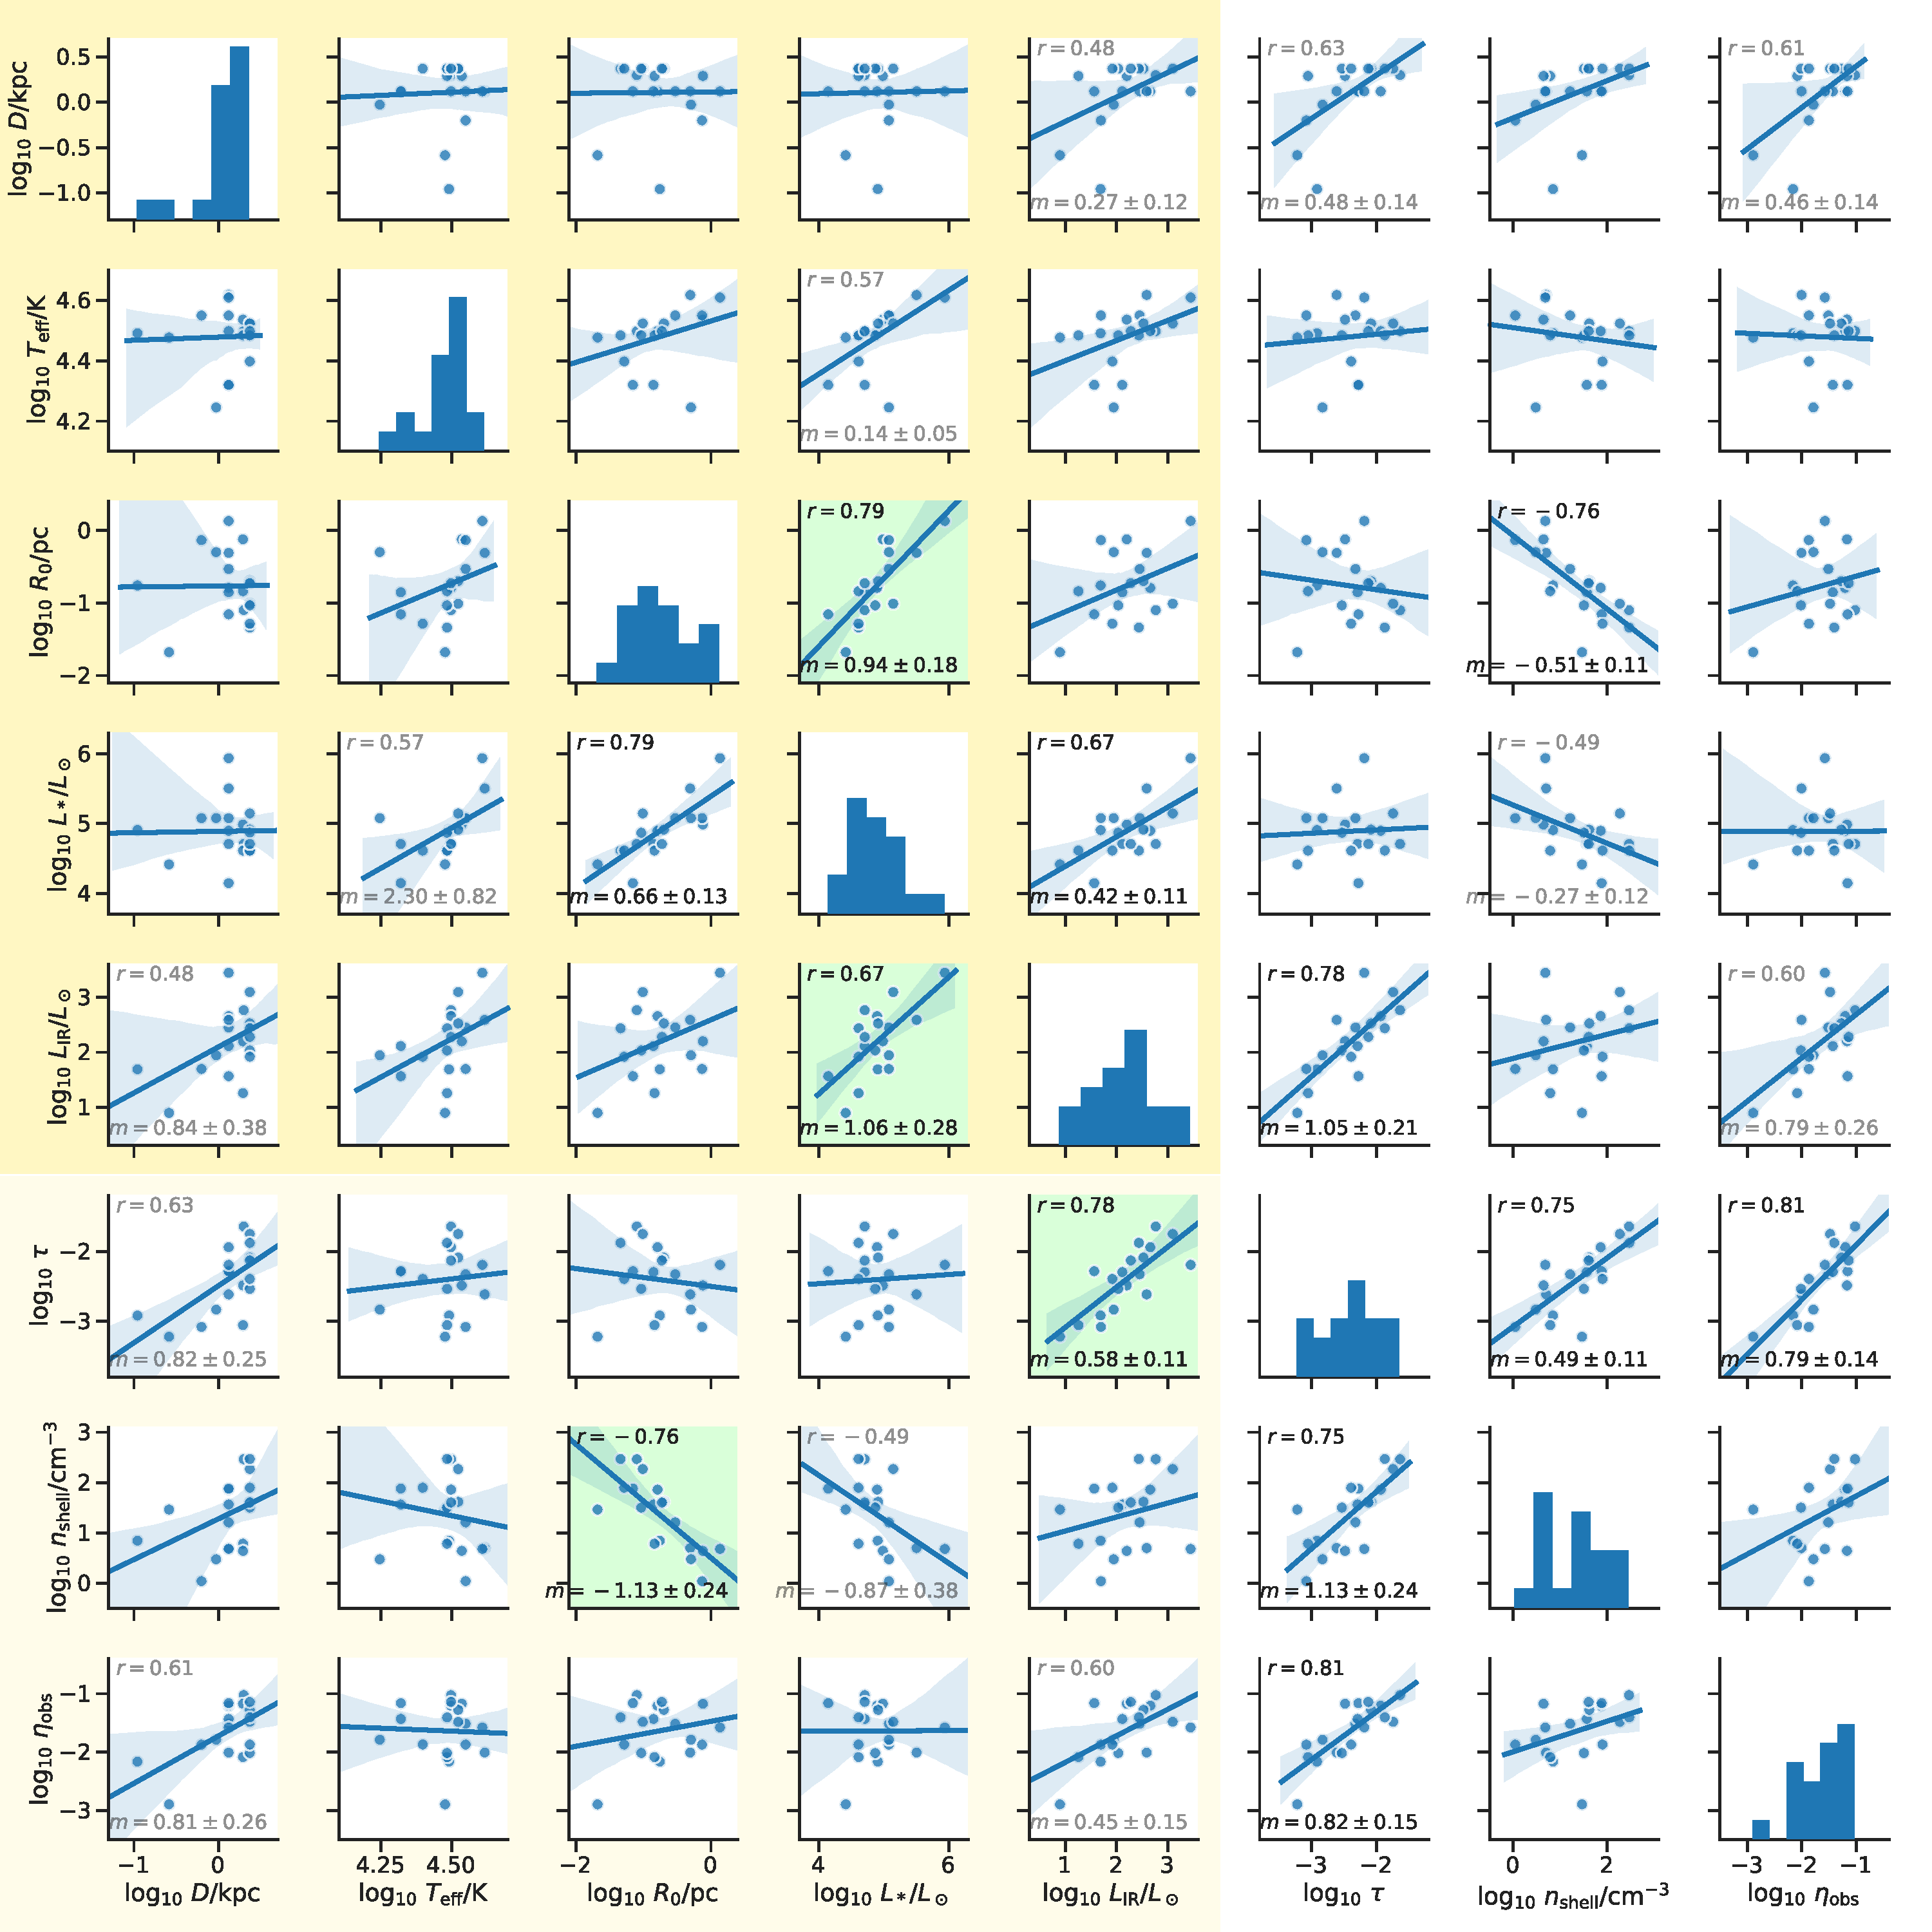
\includegraphics[width=\linewidth]{figs/K18-pairplot-edited}
%   \caption[K18 pair plot]{Pair plots of correlations between observed
%     and derived parameters of bows from the \citep{Kobulnicky:2018a}
%     sample.}
%   \label{fig:K18-pairplot-edited}
% \end{figure*}


\begin{figure}
  \centering
  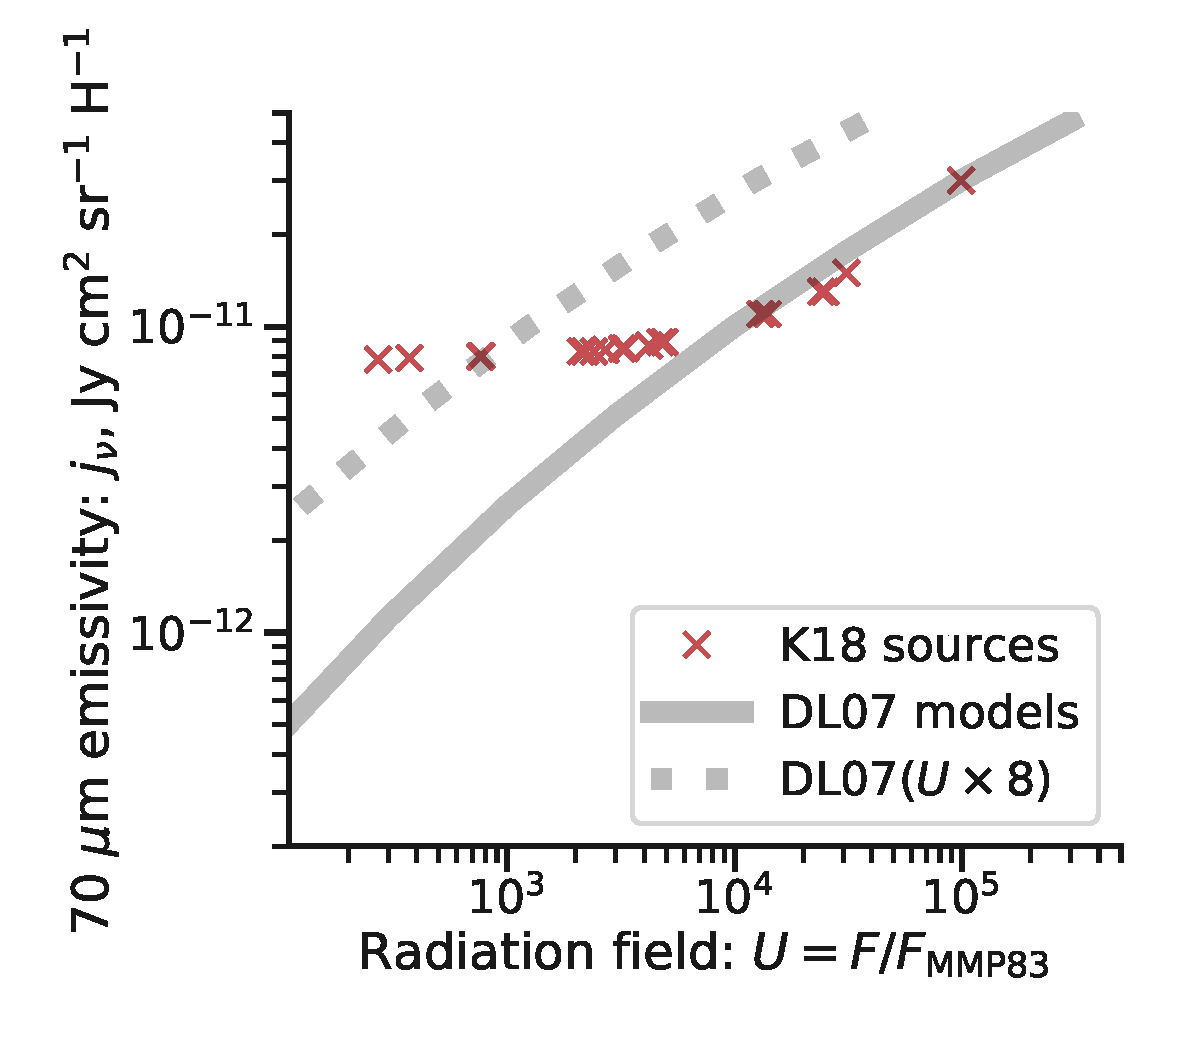
\includegraphics[width=\linewidth]{figs/K18-emissivity-vs-U}
  \caption{Discrepancies in \SI{70}{\um} emissivities that we have
    identified in K18.  Red crosses show the emissivities given in
    K18's Table~2 as a function of the radiation field \(U\), while
    the solid gray line shows the emissivities that they claim to be
    using from \citet{Draine:2007a}.  The dashed line shows the
    emissivities that we believe they should have been using, which
    correct for the marked difference in spectral energy distribution
    between OB stars and the Galactic interstellar radiation field
    (see App.~\ref{sec:grain-temp-emiss}).}
  \label{fig:k18-emissivity}
\end{figure}

\newcommand\LOS{\ensuremath{_{\text{los}}}}
K18 derive mass loss rates for their sources using a method that is
different from the one that we employ in
\S~\ref{sec:summary-discussion}.  Both methods are based on
determining the stellar wind ram pressure that supports the bow shell,
but K18 do so via the following steps:
\begin{enumerate}[K1.]
\item \label{K1} The line-of-sight mass column through the shell is
  calculated by combining the peak surface brightness at \SI{70}{\um},
  \(S_{70}\), with a theoretical emissivity per nucleon,
  \(j_{70}(U)\), from \citet{Draine:2007a}:
  \(\Sigma\LOS = S_{70} / \bar{m} j_{70}(U)\).  This depends on
  knowledge of the stellar radiation field at the shell:
  \(U \propto L_* / R_0^2\).
\item \label{K2} The shell density is found from the line-of-sight
  mass column using an observationally determined ``chord diameter'',
  \(\ell\), which is assumed to be equal to the depth along the line
  of sight: \(\rho\shell = \Sigma\LOS / \ell\).
\item \label{K3} The internal ram pressure is equated to the external
  ram pressure, which is found by assuming a stream velocity of
  \SI{30}{km.s^{-1}} and a compression factor of 4 across the outer
  shock:
  \(P_{\text{stream}} = 0.25 \rho\shell \times
  (\SI{30}{km.s^{-1}})^2\).
\end{enumerate}
There are clear parallels but also differences between steps
K\ref{K1}--K\ref{K3} and our own steps P\ref{P1}--P\ref{P3}.  Our
step~P\ref{P1} depends on the total observed infrared flux of the bow
combined with an assumption about the grain opacity at ultraviolet
wavelengths, while step~K\ref{K1} depends on the peak brightness at a
single wavelength combined with an assumption about the grain
emissivity at infrared wavelengths.  Our step~P\ref{P2} requires an
assumption about the relative thickness of the shell, while
step~K\ref{K2} is more directly tied to observations.\footnote{%
  Note that there is a relation between the chord length, \(\ell\),
  and the shell thickness, \(h\shell\), but this depends on the
  planitude, \(\Pi\) of the bow shape \citep{Tarango-Yong:2018a}:
  \( h\shell/R_0 = \Pi \bigl(1 - \{1 - [\ell/(2 \Pi R_0)]^2\}^{1/2}\bigr)\).  } %
On the other hand, step~K\ref{K3} makes a roughly equivalent
assumption about the shock compression factor,\footnote{%
  In reality, the compression factor may be larger or smaller than 4,
  depending on the efficiency of the post-shock cooling (see
  \S~\ref{sec:radi-cool-lengths}).  For instance, for
  \(v = \SI{30}{km.s^{-1}}\) as assumed by K18 and \(T = \SI{e4}{K}\),
  one has a Mach number of \(\M_0 = 2.63\) and a compression factor of
  2.8 for a non-radiative shock (by eq.~[\ref{eq:shock-n-jump}]) or a
  factor of \(\M_0^2 =6.9\) for a strongly radiative one.  } %
and a further assumption about the stream velocity. These assumptions
are not necessary for our step~P\ref{P3}, but we do need to assume a
value for the shell gas temperature.

In principle, both methods are valid and their different assumptions
and dependencies on observed quantities and auxiliary parameters
provide an important cross check on one another.  However, as
explained in detail in Appendix~\ref{sec:grain-temp-emiss}, the
\(j_\nu(U)\) relation depends on the shape of the illuminating SED,
which means that the \citet{Draine:2007a} models require modification
when applied to grains around OB stars.  In addition, when attempting
to replicate the K18 values of \(j_{70}\) we find that they only
follow the \citet{Draine:2007a} values for \(U > \num{e4}\), tending
to a constant value for weaker radiation fields.  The situation is
summarized in Figure~\ref{fig:k18-emissivity}, where the values taken
directly from Table~2 of K18 are shown by red crosses, the values they
claim to be using are shown by the gray solid line (this curve is
consistent with that shown in K18 Fig.~2), and the values they
\textit{should} have been using are shown by the gray dashed line.

% If we replaced K3 with M3, then mass loss rates would be reduced by 1.86 across the board

\begin{figure}
  \centering
  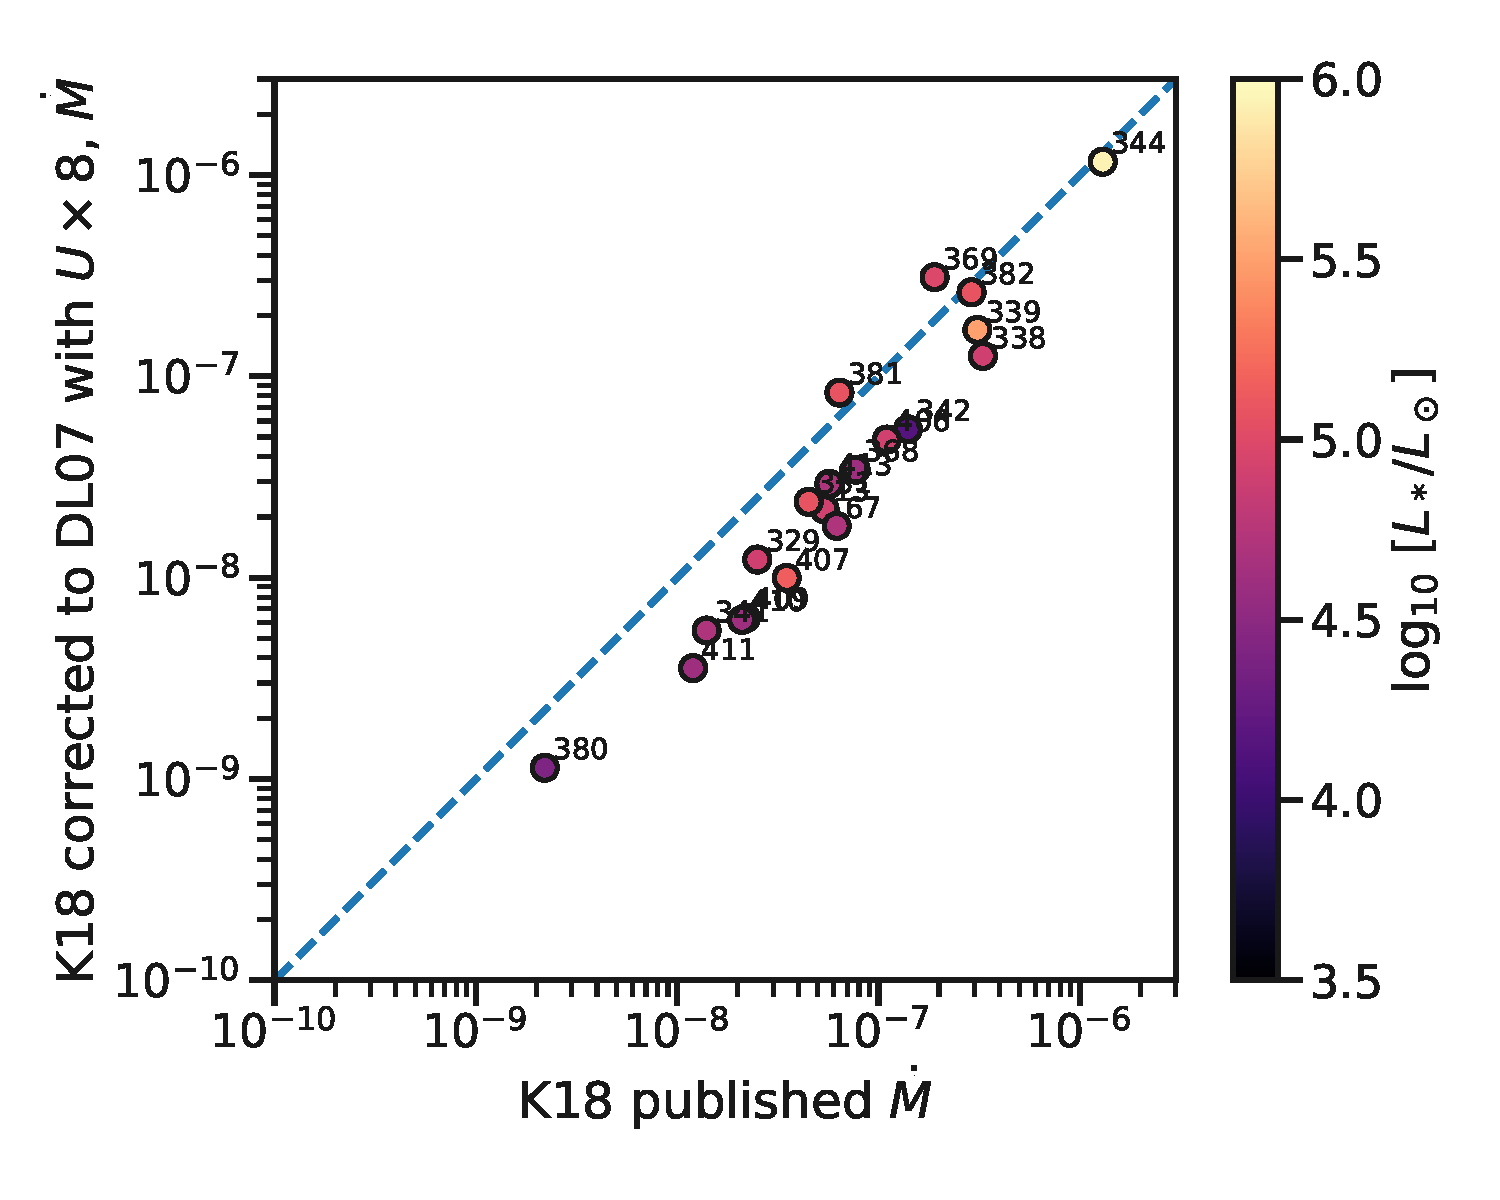
\includegraphics[width=\linewidth]{figs/K18-mdot-Ux8-comparison}
  \caption{Effects on mass-loss determination of correcting the K18
    emissivities.  The mass-loss rates from Table~2 of K18 are shown
    on the \(x\) axis, while the corrected values are shown on the
    \(y\) axis.  Symbols are color coded by the strength of the
    radiation field, \(U\). The corrected mass-loss rates are
    predominantly lower by a factor of roughly 2.}
  \label{fig:k18-mdot-corrected-emissivity}
\end{figure}

After correcting the \SI{70}{\um} emissivities in this way, we
re-derive the mass loss rates, following the same steps as in K18,
which are then used in Figure~\ref{fig:mass-loss-vs-luminosity}b of
\S~\ref{sec:summary-discussion}.  The difference between these
corrected mass-loss rates and those published in K18 is shown in
Figure~\ref{fig:k18-mdot-corrected-emissivity}.  It can be seen that
sources with \(U \approx \num{e3}\) (darker shading) are relatively
unaffected but that sources with stronger radiation fields (lighter
shading) have their mass-loss increasingly reduced, as could be
surmised from Figure~\ref{fig:k18-emissivity}.  The average reduction
is by a factor of about two.

\begin{figure}
  \centering
  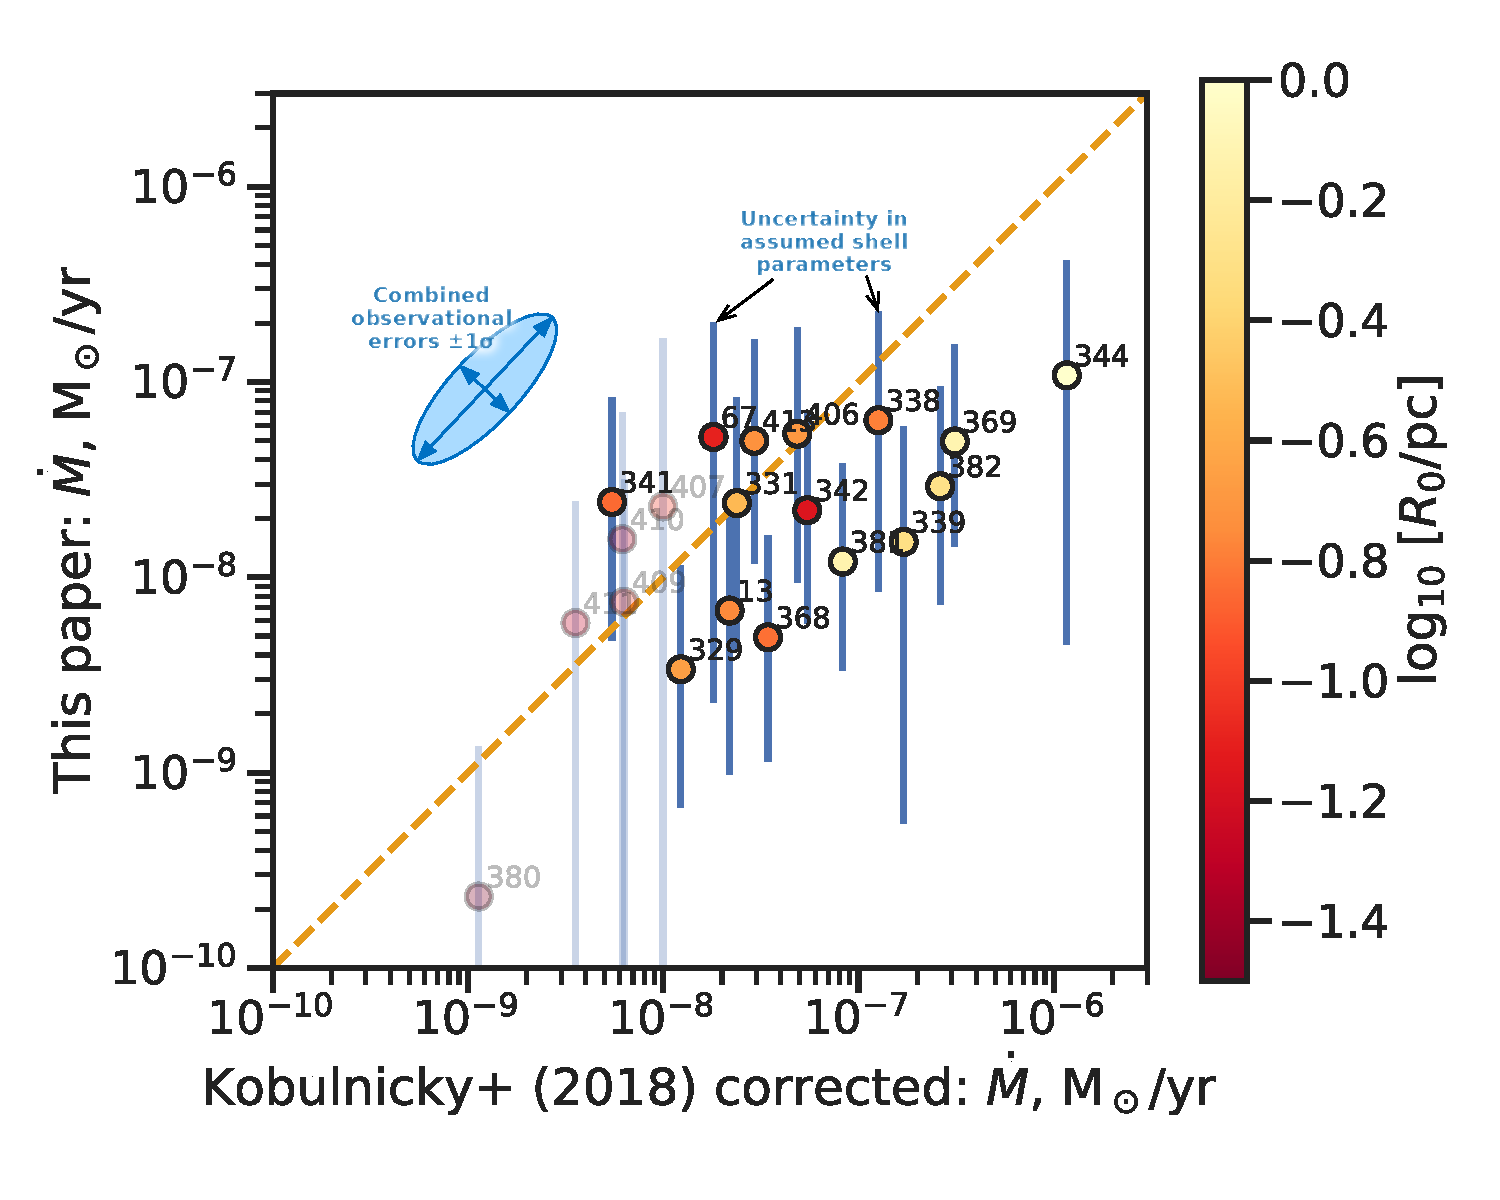
\includegraphics[width=\linewidth]{figs/K18-mdot-corrected-comparison-R0-edited}
  \caption{Comparison of the two mass-loss methods: K18 corrected
    method (\(x\) axis) versus our method (\(y\) axis).  Error bars on
    the \(y\) axis correspond to a factor-three uncertainty in
    \(\eta\shell\).  Sources for which these error bars overlap with
    the RBW zone are only upper limits for the wind mass-loss rate,
    and are indicated by faint symbols.}
  \label{fig:mass-loss-comparison}
\end{figure}

Finally, in Figure~\ref{fig:mass-loss-comparison} we compare our own
mass-loss determinations with the corrected K18 values.  The plot
symbols are shaded according to the physical size of the bow, \(R_0\).
It is apparent that the two methods are broadly in agreement on
average, but there is considerable dispersion for individual objects,
with only a weak correlation between the results of the two techniques
(Pearson correlation coefficient \(r = 0.67\)).  Interestingly, the
smaller bows (darker shading) show much better agreement than the
larger bows (lighter shading).  The five bows with
\(R_0 > \SI{0.4}{pc}\) (339, 344, 369, 381, 382) show a difference of
nearly an order of magnitude, in the sense that our method
consistently predicts lower mass-loss rates than K18.  For a further
five of the sources (380, 407, 409, 410, 411), our method gives only
an upper limit to the wind mass-loss rate if one assumes a
factor-three uncertainty in \(\eta\shell\), and these bows are among
the smallest in the sample, all with \(R_0 < \SI{0.1}{pc}\).

\subsection{Uncertainty estimates for observational quantities}
\label{sec:uncert-estim-observ}

In this section, we estimate the \(1\sigma\) uncertainties in
observational measurements, which contribute to the uncertainties in
the derived quantities: \(\tau\), \(\eta\), and \(\dot M\) (see
\S~\ref{sec:summary-discussion}).

\subsubsection{Distance}
\label{sec:distance}

Most sources are members of known high-mass clusters with distance
uncertainties less than 20\% (0.08~dex). The only exception is
Source~329 in Cygnus, for which the distance uncertainty is roughly a
factor of 2 \citep{Kobulnicky:2018a}.

\subsubsection{Stellar luminosity}
\label{sec:stellar-luminosity}

The stellar luminosity is determined from spectral classification,
which makes it independent of distance.  Taking a \SI{2000}{K}
dispersion in the effective temperature scale \citep{Martins:2005a}
gives an uncertainty of 25\% in the luminosity, and adding in possible
errors in gravity and the effect of binaries, we estimate a total
uncertainty in \(L_*\) of 50\% (0.45~mag or 0.18~dex).

\subsubsection{Shell flux and surface brightness}
\label{sec:shell-flux-surface}

We estimate the uncertainty in shell bolometric flux,
\(F_{\text{IR}}\), by comparing two different methods: model fitting
\citep{Kobulnicky:2017a} and a weighted sum of the 8, 24, and
\SI{70}{\um} bands (eq.~[\ref{eq:total-ir-flux}]), giving a standard
deviation of 17\% (0.07~dex).  To this, we add the estimate of 25\%
for the effects of background subtraction uncertainties on individual
photometric measurements \citep{Kobulnicky:2017a}. The absolute flux
calibration uncertainty for both Herschel PACS \citep{Balog:2014a} and
Spitzer MIPS \citep{Engelbracht:2007a} is less than 5\%, which is
small in comparison. Combining the 3 contributions in quadrature gives
a total uncertainty of 0.12~dex.  We adopt the same uncertainty for
the \SI{70}{\um} surface brightness.

\subsubsection{Angular sizes}
\label{sec:angular-sizes}

For the angular apex distance, \(\theta\), the largest uncertainty for
well-resolved sources is due to the unknown inclination.
\citet{Tarango-Yong:2018a} show that the dispersion in true to
projected distances can introduce an uncertainty of \(30\%\)
(0.11~dex) in unfavorable cases (e.g., their Fig.~26).  For 5 of the
20 sources from \citet{Kobulnicky:2018a}, \(\theta\) is of order the
Spitzer PSF width at \SI{24}{\um}, so the errors may be larger.

\subsubsection{Stellar wind velocity}
\label{sec:stell-wind-veloc}

Although this is not strictly an observed quantity for the K18 sample,
we will treat it as such since it is estimated per star, based on the
spectral type.

\subsubsection{Uncertainties and covariance for derived quantities}
\label{sec:comb-uncert-covar}

\begin{table}
  \centering
  \caption[Derived]{Propagation of observational uncertainties to derived quantities}
  \label{tab:derived-parameters}
  \setlength\tabcolsep{3pt}
  \begin{tabular}{l S S S S S S}
    \toprule
    \(x_i\) & {\(\sigma_{x_i}\)}
    & {\(\Delta_{x_i} (\tau)\)} & {\(\Delta_{x_i} (\eta\shell)\)}
    & {\(\Delta_{x_i} (\dot M)\)} & {\(\Delta_{x_i} (\dot M_{\text{K18}})\)}
    & {\(\Delta_{x_i} (L_*)\)}
    \\
    \midrule
    \(D\)     & 0.08 & 2  & 3 & 3 & 2 & 0\\
    \(L_*\)   & 0.18 & -1 & -2 & -1 & -0.5 & 1\\
    \(F\IR\)  & 0.12 & 1 & 1 & 1 & 0 & 0\\
    \(I_{70}\) & 0.12 & 0 & 0 & 0 & 1 & 0\\
    \(\theta\) & 0.11 & 0 & 1 & 1 & 2 & 0\\
    \(\ell/R\) & 0.08 & 0 & 0 & 0 & -1 & 0\\
    \(V\wind\) & 0.18 & 0 & 0 & -1 & -1 & 0\\
    \bottomrule
  \end{tabular}
\end{table}



Even though errors in the fundamental observed quantities, \(x_i\),
are assumed independent, errors in the derived quantities,
\(f_k(x_1, x_2, \dots)\), will not necessarily be so.  For the
purposes of this paper:
\begin{align}
  \label{eq:observed-and-derived}
  x_i \in &  \left\{D;\ L_*;\ F\IR;\ I_{70};\ \theta;\ \ell/R;\ V\wind \right\} \\
  f_k \in & \left\{\tau;\ \eta\shell;\ \dot M;\ \dot M_{\text{K18}};\ L_* \right\}
            \ .
\end{align}
Note that \(L_*\) appears in both lists because we use it as a graph
axis in Figure~\ref{fig:mass-loss-vs-luminosity}.  For the case where
each \(f_k\) is a simple product of powers of the \(x_i\), the
propagation of errors reduces to linear algebra of log
quantities. This is exactly true for \(\tau\) and \(\eta\shell\), but
only approximately so for \(\dot M\) and
\(\dot M_{\text{K18}}\).\footnote{%
  For \(\dot M\) it is true for \(\eta\shell \gg 1.25 \tau\) and for
  \(\dot M_{\text{K18}}\) it is true in the limit that the grain
  emissivity can be expressed as a power law in \(U\).} %
We define \(\Delta_{x_i} (f_k)\) as the logarithmic derivative
\(d \ln f_k / d \ln x_i \) and \(\sigma_{x_i}\) as the rms dispersion
in \(x_i\), measured in dex.  These are given in
Table~\ref{tab:derived-parameters}.  Then, the elements of the
variance--covariance matrix for the derived parameters are
\begin{equation}
  \label{eq:covariance}
  C_{k,k'} = \sum_{i} \Delta_{x_i} (f_k) \, \sigma_{x_i}^2 \, \Delta_{x_i} (f_{k'}) \ , 
\end{equation}
which are given in Table~\ref{tab:covariance}, assuming the
\(\sigma_{x_i}\) derived in
\S~\ref{sec:distance}--\ref{sec:stell-wind-veloc} as suitable for the
K18 sources.  It can be seen that many of the off-diagonal elements
are of similar magnitude to the diagonal elements, which is an
indication of significant correlations between the errors in the
different parameters.

\begin{table}
  \centering
  \caption[Covariance]{Variance--covariance matrix \(C_{k,k'}\) for derived quantities}
  \label{tab:covariance}
  \setlength\tabcolsep{3pt}
  \begin{tabular}{l S S S S S }
    \toprule
    & {\(\tau\)} & {\(\eta\shell\)}
    & {\(\dot M\)} & {\(\dot M_{\text{K18}}\)} & {\(L_*\)}
    \\
    \midrule
    \(\tau\)               &  0.0724 &  0.1176 &  0.0852 &  0.0418 & -0.0324 \\
    \(\eta\shell\)         &  0.1176 &  0.2137 &  0.1489 &   0.095 & -0.0648 \\
    \(\dot M\)             &  0.0852 &  0.1489 &  0.1489 &  0.1112 & -0.0324 \\
    \(\dot M_{\text{K18}}\)&  0.0418 &   0.095 &  0.1112 &  0.1353 & -0.0162 \\
    \(L_*\)                & -0.0324 & -0.0648 & -0.0324 & -0.0162 &  0.0324 \\
    \bottomrule
  \end{tabular}
\end{table}

For any particular pair of derived quantities, \(f_m\) and \(f_{n}\),
one can find the \textit{error ellipse} that characterises the
projection of observational errors onto the \(f_m\)--\(f_{n}\) plane.
The ellipse can be described by standard deviations along major and
minor axes, \(\sigma_a\), \(\sigma_b\), together with the angle
\(\theta_a\) between the \(f_m\) axis and the ellipse major axis.
These are given via the eigenvalues and eigenvectors of the relevant
\(2 \times 2\) submatrix of the covariance matrix:
\begin{align}
  \label{eq:error-ellipse}
  \sigma_a^2 = & \frac12 \left\{   C_{m,m} + C_{n,n}
                 + \left[ \left( C_{m,m} + C_{n,n} \right)^2
                 - 4 C_{m,n}^2 \right]^{1/2}\right\} \\
  \sigma_b^2 = & \frac12 \left\{   C_{m,m} + C_{n,n}
                 - \left[ \left( C_{m,m} + C_{n,n} \right)^2
                 - 4 C_{m,n}^2 \right]^{1/2}\right\} \\
  \theta_a = & \frac12 \arctan \left( \frac{2 C_{m,n}}{C_{m,m} - C_{n,n}} \right) \ .
\end{align}
For instance, Table~\ref{tab:error-ellipse} shows the resultant error
ellipse parameters for the relations plotted in
Figures~\ref{fig:All-sources-eta-tau} and
\ref{fig:mass-loss-vs-luminosity}ab, which are shown in blue on the
respective graphs.

\begin{table}
  \centering
  \caption[Error ellipse]{Error ellipse parameters for particular pairs of derived quantities}
  \label{tab:error-ellipse}
  \begin{tabular}{l l S S S l}
    \toprule
    \(f_m\) & \(f_n\) &  {\(\sigma_a\)} & {\(\sigma_b\)}
    & {\(\theta_a\), \si{\degree}} & Figure   \\
    \midrule
    \(\tau\) & \(\eta\) & 0.529 & 0.077 & 60.5 & \ref{fig:All-sources-eta-tau} \\
    \(L_*\) & \(\dot M\) & 0.397 & 0.155 & -75.5 & \ref{fig:mass-loss-vs-luminosity}a \\
    \(L_*\) & \(\dot M_{\text{K18}}\) & 0.371 & 0.173 & -81.3 & \ref{fig:mass-loss-vs-luminosity}b \\
    \(\dot M_{\text{K18}}\) & \(\dot M\) & 0.503 & 0.175 & 46.7 & \ref{fig:mass-loss-comparison} \\
    \bottomrule
  \end{tabular}
\end{table}


\begin{figure}
  \centering
  \footnotesize
  \begin{verbatim}
import numpy as np
sigx = np.diag([0.08, 0.18, 0.12, 0.12, 0.11, 0.08, 0.18])
Dfx = np.array([
    [2, -1, 1, 0, 0, 0, 0],
    [3, -2, 1, 0, 1, 0, 0],
    [3, -1, 1, 0, 1, 0, -1],
    [2, -0.5, 0, 1, 2, -1, -1],
    [0, 1, 0, 0, 0, 0, 0]
])
C = Dfx @ sigx**2 @ Dfx.T
  \end{verbatim}
  \caption{Snippet of Python code that calculates the
    covariance matrix of Table~\ref{tab:covariance}.  The last line
    implements equation~\eqref{eq:covariance} by a triple matrix
    product of the derivatives matrix \texttt{Dfx}, the square of a
    diagonal matrix of observational standard deviations \texttt{sigx},
    and the transpose of \texttt{Dfx}.}
  \label{fig:python-covar}
\end{figure}


%%% Local Variables:
%%% mode: latex
%%% TeX-master: "dusty-bow-wave"
%%% End:
